\chapter{Neural Networks overview}
\label{appendix:neuralNetworks}
We provide an overview of the main concepts and techniques relating to Neural Networks as are 
important for this work. Section~\ref{appendix:fundamentalsNN} and~\ref{appendix:recurrentNN} 
are based on Graves~\cite{seqlab:Graves2012-385} work description for Supervised Sequence 
Labeling with Recurrent Networks and Section~\ref{appendix:convolutionalNN} is based 
on~\cite{appendix:OSheaN15}.

\section{Neural Networks Fundamentals}
\label{appendix:fundamentalsNN}
Artificial Neural Networks (ANNs), or simply Neural Networks (NNs), are mathematical models 
inspired by how biological brains process information. Their basic structure is a network of 
small processing units, also seen as nodes, joined to each other by weighted connections. 
Similar to how synapses work in biological neurons, the network is activated by providing an 
input to some or all nodes, which spreads this activation throughout the rest of the network 
along the weighted connections.

\subsection{Multilayer Perceptrons}
Among the different varieties of neural networks, \textbf{Feedforward Neural Networks} are 
structured in an acyclic way, meaning their connections do not form a cycle. One example are 
the multilayer perceptrons (MLP), which are arranged in layers with connections feeding 
forward from one layer to the next. An illustration can be seen in Figure~\ref{fig:multilayerPerceptron}, 
where input data are passed to an \textbf{input layer} and then propagated through one or more 
\textbf{hidden layers} to the final \textbf{output layer}. This kind of architecture is more 
suitable for classification or function approximation tasks~\cite{seqlab:Graves2012-385}.

\begin{figure}[!h]
    \centering
    
\includegraphics[scale=.45]{imagenes/insertImage.png}
    \caption{Multilayer perceptron [ref].}
    \label{fig:multilayerPerceptron}
\end{figure}

The process to pass data through layers is known as the \textbf{forward pass} of the network. 
Given an input vector of length $I$, an input layer of the same length would receive this 
input vector where each unit in the input layer calculates a weighted sum. For a hidden unit 
$h$, we refer to this sum as the network input to unit $h$, denote as $a_h$. Denoting $w_{ij}$ 
as the weight from unit $i$ to unit $j$, the formula of $a_h$ for a layer $H_{l}$ is calculated 
using the formula in Equation~\ref{eq:hiddenState}.

\begin{equation} \label{eq:hiddenState}
    a_h = \sum_{h' \in H_{l-1}}^I w_{h'h} \; b_{h'}
\end{equation}

where $b_{h'}$ corresponds to the final activation function of the previous layer. The $b_h$ 
value is calculated by applying an activation function $\theta_h$ over $a_h$, as seen in 
Equation~\ref{eq:finalActivation}. Note that for the first hidden layer, the previous layer 
is the input layer.

\begin{equation} \label{eq:finalActivation}
    b_h = \theta_h(a_h)
\end{equation}

This activation function $h$ can vary, though some of the most common functions used are the 
hyperbolic tangent~\ref{eq:tanh} or sigmoid~\ref{eq:sigmoid} functions. Two important features 
about activation functions: they are non-linear and differentiable. Non-linearity allows the 
network to build more complex internal features (e.g. build more flexible boundaries in a 
classification task), and differentiability is required to perform the backward pass that 
will be mentioned below.

\begin{equation} \label{eq:tanh}
    tanh(x) = \frac{e^{2x}-1}{e^{2x}+1}
\end{equation}
\begin{equation} \label{eq:sigmoid}
    sigmoid(x) = \frac{1}{1+e^{-x}}
\end{equation}

This process of summation and activation is repeated for $L$ hidden layers until reaching the 
output layer, where the output vector $y$ is determined by using the activation of the last 
hidden layer $H_L$. Then, the network input $a_k$ to each output unit $k$ is calculated by 
summing over the units of the connected to it, the same way as is expressed in Equation~\ref{eq:hiddenState}. 
The output activation function to be used depends on the task the network aims to fulfill. 
For simple binary classification, the sigmoid function~\ref{eq:sigmoid} is applied since its 
values between 0 or 1 can be seen as a binary probability $p(z|x)$, with $z$ being the target 
vector. Furthermore, if the classification task includes more than 2 classes, there is a 
convention to have $K$ output units, and normalize the output activations with the softmax 
function~\ref{eq:softmax}. Therefore, the class probability for $C_k$ given the output $x$ is 
represented by Equation 5

\begin{align} \label{eq:softmax}
    p(C_k|x) & = y_k \nonumber \\
        & = softmax(a_k) \nonumber \\ 
        & = \frac{e^{a_k}}{\sum_{k'=1}^K e^{a_{k'}}}
\end{align}

Lastly, a 1-to-K scheme is used to represent the target class $z$ where $z$ is represented as 
a one-hot vector (e.g. if $K=4$, the class $C2$ is represented as $[0, \; 1, \; 0, \; 0]$). 
More formally, the way to express the target probabilities are as follows:

\[
    p(z|x) = \prod_{k=1}^K y_k^{z_k}
\]

In the context of pattern classification, the class label that should be chosen corresponds to 
the most active output unit, i.e. the higher value from all target probabilities.

\subsection{Network Training}
In order to have an idea whether a neural network is working as expected, a loss function is 
used. As per activation functions, the loss function to be used depends on the task the Neural 
Network is performing.  For example, for multiple classification the maximum-likelihood function 
is commonly used as a loss function~\cite{appendix:bishop1995neural}:

\[
    L(y_k, z) = \sum_{k=1}^K z_k ln \; y_k
\]

Neural networks are able to learn, i.e. they can generalize to unseen data, so they can be 
trained by minimizing the loss function L. One of the simplest algorithms to perform such 
training process is the \textit{gradient descent} algorithm. \text{Gradient descent} consists 
of repeatedly taking a small, fixed-size step in the direction of the negative error gradient 
of the loss function, which can also be seen as going in the opposite direction of the 
negative slope of the loss function. Note that we perform gradient descent over a training 
dataset, while we save a test dataset that is not used to train but to evaluate the overall 
performance after training.

Thus, a weight update $\Delta w^n$, also known as gradient , is used to update the the weight 
vector $w^n$ from the $n^{th}$ network layer. The gradient $\Delta w^n$ consists of the 
partial derivative of the loss function when the weight vector $w^n$ varies. This derivative 
is adjusted by a \textbf{learning rate} $\alpha \in [0, 1]$ which limits how quick the training process 
is converging. Then, on each gradient descent iteration $i$ the weight vector $w^n$ is updated as 
follows:

\[
    w_{i}^n = w_{i-1}^n - \Delta w_{i-1}^n = w_{i-1}^n - \alpha \frac{\partial L}{\partial w_{i-1}^n}
\]

The backpropagation technique is commonly used to calculate these 
gradients~\cite{appendix:rumelhart1985learning, appendix:williams1995gradient, appendix:werbos1988generalization}, 
often referred to as the \textbf{backward pass} of the network. Backpropagation consists of 
the repeated application of chain rule for partial derivatives. For example, for a multiclass 
network, the application of the chain rule over the loss function defined as 
$\frac{\partial L(x, z)}{\partial w_{ij}} = \frac{\partial L(x, z)}{\partial a_j} \frac{\partial a_j}{w_{ij}}$, 
which then can be deduced by applying the chain rule again over the unknown gradients. 
Note that this process has to be performed over every weight of each layer on the network.

The training algorithm is repeated until a \textbf{stopping criteria} is met (e.g. stop after 
a fixed amount of steps, when reaching a certain loss threshold, or when failing to reduce the 
loss on a given number of consecutive steps). Usually, this process involves using the entire 
training data more than one time, where an entire pass over the data is known as one \textbf{epoch}. 
By the end of the training process, we expect to have the neural network’s weights such that 
the loss function has reached a value as close as possible to the global minimum when 
evaluating over test examples (i.e. it can predict as best as possible over the training data).

The training process involves many issues that can lead to bad performance, a long time to 
train models, or divergence problems (i.e. training process never ends). One common issue is 
when the gradient descent process gets stuck in local minimums, which can be addressed by 
adding a momentum term to reduce learning inertia~\cite{appendix:plaut1986experiments}. To 
boost training time, many variants of gradient descent have been proposed such as stochastic 
gradient descent or mini-batch gradient descent~\cite{appendix:lecun1998efficient}.

Another issue related with bad performance is \textbf{overfitting}, which causes the network 
not to be able to generalise properly since it \textit{“memorizes”} the data from the training 
dataset. One way to see if a model is overfitted is to check the loss function values 
evolution over the training process for the training and the test set: if the loss for the 
test is not decreasing but instead increasing while the loss for the training set is 
constantly decreasing, the model is getting overfitted.

\begin{figure}[!h]
    \centering
    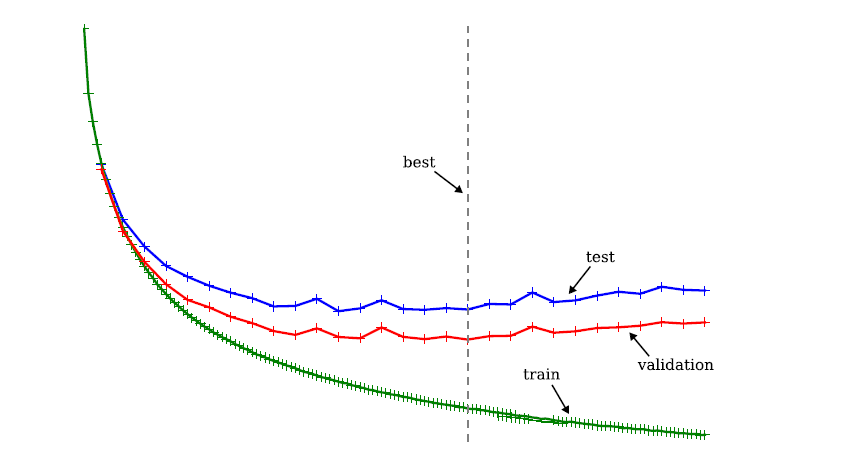
\includegraphics[scale=.45]{imagenes/appendices/appA_overfitting.PNG}
    \caption{Example of early stopping analysis using validation data~\cite{seqlab:Graves2012-385}.}
    \label{fig:earlyStopppingExample}
\end{figure}

One solution that helps to address the overfitting issue is to use a small portion of the 
training set as a validation set to include an \textbf{early stopping criteria}. This 
validation set is not used to train the network but to perform validation steps every certain 
amount of training steps. Then, the loss values for the validation steps are used to decide 
when to stop training. For example, Figure~\ref{fig:earlyStopppingExample} shows the losses 
over all three data sets (train, validation, test) through the training process Then, we can 
detect that the best weight values are found just before the validation loss stops its 
decreasing tendency and start increasing again (where the “best” stripped vertical line is 
placed). There are other techniques to reduce overfitting known as regularizers based on 
input noise~\cite{appendix:an1996effects, appendix:koistinen1991kernel, appendix:bishop1995neural} 
or weight noise~\cite{appendix:murray1994enhanced,appendix:jim1996analysis}.

Though most of the performance of ANNs relies on learnable parameters (such as layers’ weights), 
there are other parameters that can be set manually to improve the model’s performance, also 
known as \textbf{hyperparameters}. Some hyperparameters could be the number of hidden layers, 
the number of hidden units per layer, the learning rate, among others.

Lastly, it is also important to understand how the network input is represented. When we 
mention the \textbf{input representation}, we refer to the representation of the information 
required to predict the outputs, such as the input vector or the network weights. One 
procedure is input standardisation, which consists of normalizing the components of the input 
vectors to have mean 0 and standard deviation 1 over the training set. This standardization 
does not alter the information but helps to improve performance by limiting the values of the 
input vector to a more suitable range for a standard activation function~\cite{appendix:lecun1998efficient}. 
Note that the validation set and test set have to be standardised using the same distribution 
used for the training set. 

Another procedure is \textbf{weight initialisation}, which helps gradient descent to 
\textit{“break symmetry”} between units~\cite{appendix:lecun1998efficient} and avoid training 
divergence. Weight initialisation then is to initialise weights with either a random 
distribution in the range of small values or a Gaussian distribution with mean 0 and 
standard deviation 0.1.

After reviewing the fundamental concepts needed to understand how neural networks are 
structured and trained, we will review two neural networks architectures used in this work: 
Recurrent Neural Networks and Convolutional Neural Networks.

\section{Recurrent Neural Networks}
\label{appendix:recurrentNN}
A Recurrent Neural Network (RNN) is a generalization of traditional feedforward Neural 
Networks that allows cyclical connections~\cite{seqlab:Graves2012-385}. While MLPs can only 
map from input to output vectors, RNNs can map the entire history of previous inputs to an 
output. Hence, RNN connections allow the network to have “memory” of previous inputs, thus 
influencing the network output. Furthermore, RNNs are more fit for tasks involving sequence 
data, such as text or audio. An example of a RNN architecture can be seen in Figure 1.

\begin{figure}[!h]
    \centering
    
\includegraphics[scale=.45]{imagenes/insertImage.png}
    \caption{Recurrent Neural Network architecture example.}
    \label{fig:recurrentNN}
\end{figure}

A standard RNN computes the \textbf{forward pass} the same way as an MLP with a single hidden 
layer, with the difference that the activations arrive at the hidden layer from both the 
current external input and the hidden layer activations from the previous time step. Given a 
sequence of inputs $(x_1,\ldots,x_T)$, with $T$ the input length, the forward pass for an RNN 
with $I$ input units and $H$ hidden units is computed using the following formula:

\begin{equation} \label{eq:hiddenStateRNN}
    a_h^t = \sum_{i=1}^I w_{ih} \; x_i^t + \sum_{h'=1}^H w_{h'h} \; b_{h'}^{t-1}	
\end{equation}

where $x_i^t$ denotes the value of input $i$, $a_j^t$ is the network input to unit $j$, and 
$b_j^t$ is the activation unit of unit $j$, all three at time t. Then, the non-linearity $h$ 
is applied the same way as for an MLP, where functions such as the sigmoid function or 
softmax function are again a common choice:

\begin{equation} \label{eq:activationRNN}
    b_h^t = \theta_h(a_h^t)
\end{equation}

The entire learning process for RNNs is then summarized as a recursive application of the 
Equations~\ref{eq:hiddenStateRNN} and~\ref{eq:activationRNN}, starting at $t=1$. Since 
initial values $b_i^0$ are needed, they can be initialized using the same weight 
initialization methods mentioned above. The output units $a_k$ can be calculated at the same way 
as the hidden activations:

\begin{equation} \label{eq:outputStateRNN}
    a_k^t = \sum_{h=1}^H w_{hk} \; b_{h}^{t}	
\end{equation}

Then, the final activation function also depends on the task involved. For connection 
temporal classification (CTC) tasks, such as sequence labeling or translation, it is common 
to use the softmax function~\cite{appendix:graves2006connectionist}. The CTC loss function is 
used, that is defined as the negative log probability of correctly labelling all examples in 
the training set.

The \textbf{backward pass} can be performed using a backpropagation through time (BPTT) 
algorithm~\cite{appendix:williams1995gradient, semPar:werbos1990}, which is an algorithm 
based on the standard backpropagation process but adapted to RNNs. The BPTT algorithm also 
consists of a repeated application of the chain rule, with the difference that, aside from 
the output layer, the loss function also depends on the activation of the hidden layer 
through its influence on the hidden layer at the next timestep. The derivatives can be 
calculated using the same procedure described in the Learning process subsection, but taking 
into consideration that the same weights are being reused at every timestep.

Since the classical RNN architecture only looks to past information, the \textbf{Bidirectional 
Recurrent Neural Network} (BRNN) was proposed to also include future 
context~\cite{appendix:SchusterP97}. The BRNN’s structure consists of two separate recurrent 
hidden layers, both connected to the same output layer. This idea allows a forwards and 
backwards training sequence, where the layer that performs the backward training receives the 
input sequence in the opposite direction. The output layer is not updated until both hidden 
layers have processed the entire input sequence.

\subsection{Long Short-Term Memory}
Though RNNs work well with short sentences, their performance decreases with long sentences 
that involve long term dependencies due to the \textbf{vanishing gradient} 
problem~\cite{seqlab:HochreiterS97, appendix:hochreiter2001gradient}, which occurs when the 
influence of the given input on the hidden layer (and therefore on the network output), 
either decays or explodes exponentially through the recurrent connections. In order to 
address this issue, the \textbf{Long Short-Term Memory} (LSTM) model~\cite{seqlab:HochreiterS97} 
was proposed. The LSTM model allows models to perform on tasks which require long range 
temporal dependencies, such as Sequence Labeling~\cite{seqlab:HuangXY15, seqlab:MaH16}, 
Machine Translation~\cite{nlToSparql:WuSCLNMKCGMKSJL16} or Summarization~\cite{appendix:MahasseniLT17}. 
As per RNNs, the LSTM also has a bidirectional variant, also known as 
BiLSTM~\cite{appendix:graves2005framewise,appendix:ChenC04a,appendix:ThireouR07}. 

An LSTM network is similar to a standard RNN, except that the summations units in the hidden 
layer are replaced by \textbf{memory blocks}, as shown in Figure~\ref{fig:oneCellLSTM}. This 
structure allows the memory cells to store and access information over long periods of time, 
thereby reducing the effects of the vanishing gradient problem.

\begin{figure}[!h]
    \centering
    
\includegraphics[scale=.45]{imagenes/insertImage.png}
    \caption{LSTM memory block with one cell}
    \label{fig:oneCellLSTM}
\end{figure}

The following equations presented below are the formulas used to perform the forward pass 
evaluation over an LSTM with a single memory block for a timestep $t$. For multiple blocks 
the computations are repeated for each block. The values of $w_{ij}$, $a_j^t$ and $b_j^t$ 
have the same definition used before. 

First, the \textbf{Input Gates}, denoted as $a_\iota^t$~\ref{eq:inputHidden} and 
$b_\iota^t$~\ref{eq:inputActivation}. The number of inputs 
is denoted by $I$, the number of cells in the hidden layer is $H$ and the number of memory 
cells is $C$. The gate activation function $f$ most commonly used is the sigmoid function, so 
the gate activations are between 0 (gate closed) and 1 (gate open). The weight $w_{c\iota}$ 
represent the peephole weight from cell $c$ to the input gate. The state of the cell $c$ at 
time $t$ is denoted as $s_c^t$, which is calculated using Equation~\ref{eq:cellActivation}.

\begin{equation} \label{eq:inputHidden}
    a_\iota^t = \sum_{i=1}^I w_{i\iota} \; x_i^t + \sum_{h=1}^H w_{h\iota} \; b_h^{t-1} + \sum_{c=1}^C w_{c\iota} \; s_c^{t-1}
\end{equation}
\begin{equation} \label{eq:inputActivation}
    b_\iota^t = f(a_\iota^t)
\end{equation}

Then, the \textbf{Forget Gates}, denoted as $a_\phi^t$~\ref{eq:forgetHidden} and 
$b_\phi^t$~\ref{eq:forgetActivation}. The weight $w_{c\phi}$ represents the peephole weight 
from cell $c$ to the forget gate. Besides that, other symbols are equivalent to those 
mentioned for the input gate.

\begin{equation} \label{eq:forgetHidden}
    a_\phi^t = \sum_{i=1}^I w_{i\phi} \; x_i^t + \sum_{h=1}^H w_{h\phi} \; b_h^{t-1} + \sum_{c=1}^C w_{c\phi} \; s_c^{t-1}
\end{equation}
\begin{equation} \label{eq:forgetActivation}
    b_\phi^t = f(a_\phi^t)
\end{equation}

The \textbf{Cells}, denoted as $a_c^t$~\ref{eq:cellHidden} and $s_c^t$~\ref{eq:cellActivation}. The 
cell input activation function $g$ is usually hyperbolic tangent or sigmoid.

\begin{equation} \label{eq:cellHidden}
    a_c^t = \sum_{i=1}^I w_{ic} \; x_i^t + \sum_{h=1}^H w_{hc} \; b_h^{t-1}
\end{equation}
\begin{equation} \label{eq:cellActivation}
    s_c^t = b_\phi^t \; s_c^{t-1} + b_\iota^t \; g(a_c^t)
\end{equation}

Next, the \textbf{Outputs Gates}, denoted as $a_\omega^t$~\ref{eq:outputHidden} and 
$b_\omega^t$~\ref{eq:outputActivation}. The weight $w_{c\omega}$ represent the peephole w
eight from cell $c$ to the output gate.

\begin{equation} \label{eq:outputHidden}
    a_\omega^t = \sum_{i=1}^I w_{i\omega} \; x_i^t + \sum_{h=1}^H w_{h\omega} \; b_h^{t-1} + \sum_{c=1}^C w_{c\omega} \; s_c^{t-1}
\end{equation}
\begin{equation} \label{eq:outputActivation}
    b_\omega^t = f(a_\omega^t)
\end{equation}

Finally, the \textbf{Cell Outputs}, denoted as $b_c^t$~\ref{eq:cellOutput}. The cells outputs $b_c^t$ 
are the only ones connected to the other blocks in the layer. The index h is used to refer 
to cell outputs from other blocks in the hidden layer, if they exist. As per $g$, the output 
activation function $h$ is usually hyperbolic tangent or sigmoid, though sometimes the 
identity function can be used. 

\begin{equation} \label{eq:cellOutput}
    b_c^t = b_\omega^t \; f(s_c^t)
\end{equation}


\section{Convolutional Neural Networks}
\label{appendix:convolutionalNN}
The creation of \textbf{Convolutional Neural Networks} (CNNs) responds to the need to process 
certain types of data: images~\cite{appendix:OSheaN15}. Traditional ANNs do not perform well 
when processing images since its architecture does not properly support the computational 
complexity that involves processing large images as input. Whereas a 32$\times$32 image will 
be no problem to an traditional ANN, since it will require only 1024 parameters for a single 
neuron, images tend to have more resolution. On a higher scale, an image of 1024$\times$1024 
will instead require 1,048,576 parameters, which is a substantial increase. Moreover, if we 
consider colored images (RGB), a 1024$\times$1024 RGB image would require 3,145,728 
parameters. There is then a noticeable drawback of using standard feed-forward models where 
nodes are often connected to each node from the previous layer.

Convolutional Neural Networks share many similarities with standard ANNs in the way that both 
are composed of a set of neurons that are capable of learning, where each neuron receives an 
input and performs many operations, which commonly is a scalar product followed by an 
activation function. The difference resides in that CNNs are based on the idea that the input 
is shaped as an image. This idea allows the CNN architecture to adapt to this specific type 
of data. Then, a CNN architecture is built using three different types of layers: 
convolutional layers, pooling layers and fully-connected layers (same layers used in 
traditional ANNs). Additionally, each layer is organised into three dimensions: the spatial 
dimension (width and height) and the number of channels (also as known as depth, which is not 
the same as the number of layers). An example of a CNN architecture for pattern image 
classification is shown in Figure~\ref{fig:convNet}.

\begin{figure}[!h]
    \centering
    
\includegraphics[scale=.45]{imagenes/insertImage.png}
    \caption{Convolutional Neural Network for pattern image classification.}
    \label{fig:convNet}
\end{figure}

\subsection{Convolutional layer}
A \textbf{convolution layer} is the central component of CNNs, which determines the output of 
neurons using calculations based on local regions of the input. This type of layer is based on 
learnable kernels, which define local convolution operations over the input vector. A 
convolution consists of the scalar product for each value in a kernel of dimension M$\times$N 
over a local region with the same size as the kernel used:

\begin{equation} \label{eq:convolution}
    (X \ast w)_{i, j} = \sum_{m=1}^M \sum_{n=1}^{N} X_{m, n} \cdot w_{i-m, j-n}
\end{equation}

For example, in Figure~\ref{fig:convolutionPoolingExample} the convolution is being applied 
over a 3$\times$3 pooled vector, which is the size of the kernel $w$, that is, the local 
region of the entire input vector $X$. Though these kernels usually have a small spatial 
dimensionality, they are spread along the whole input vector. Besides kernel dimension, an 
application of padding over the input vector is also possible, which is the process of 
padding the border of the input with zeros. \textbf{Padding} controls both the dimensionality 
of the output volumes and gives more relevance to the input borders. Lastly, the 
\textbf{stride} is the amount of spaces the kernel is moved between each convolution. By 
setting a stride greater than 1, it is possible to reduce the amount of overlap and thus 
reduce the dimension of the activation output.

\begin{figure}[!h]
    \centering
    
\includegraphics[scale=.45]{imagenes/insertImage.png}
    \caption{Convolution operation example.}
    \label{fig:convolutionPoolingExample}
\end{figure}

Let $N$ be the size of a input vector of size N$\times$N, $F$ the kernel F$\times$F dimension, 
$P$ the padding size, and $S$ the stride value; the final dimension of the output volume will 
be $\left\lfloor \frac{N - F + 2P}{S} + 1 \right\rfloor$. Note that, in the same way an image can be 
represented in 3 dimensions, the kernel can be extended to a third dimension by increasing 
the \textbf{number of channels}, thus giving control over the output depth of the 
convolutional layer. The number of channels, stride and padding are hyperparameters that can 
be optimised. 

Kernel values are the trainable parameters which a CNN can tuned in through the same type 
of learning process ANNs perfom. The composition of convolutional layers allows to reduce the 
dimensionality of a Neural Network in terms of learnable parameters, based on the assumption 
of parameter sharing. This assumption says that \textit{“if one region is useful to compute at 
a set spatial region, then it is likely to be useful in another region”}. The constraints of 
each activation within the output volume to the same weights and bias means a significant 
decrease in the number of parameters used in a convolution layer. Then, the backward pass for 
each neuron in the output represents the overall gradient across channels, where only a 
single set of weights is updated.

After the application of the convolution, an activation function is applied over the output 
volume. The most common choice is the rectified linear unit (ReLu) which is an elementwise 
function that given a certain threshold $\alpha$ will set all values less than $\alpha$ to 0 .

\subsection{Pooling layer}
A pooling layer aims to reduce the volume of an input representation with the purposes of 
reducing the computational complexity of the model. After each activation from a convolutional 
layer, a pooling layer can be applied to scale its dimensionality through a reducing function. 
The most common type of pooling is the max-pooling layer, which is a kernel that applies a 
MAX reduction on a local region as per a convolutional kernel. Other examples are average 
pooling, or general pooling that applies average reduction and $L_1$/$L_2$ normalization 
respectively.

Though pooling layers also include settings such as kernel size, stride or number of channels, 
they do not add learnable parameters. However, they do influences in the backward pass to 
calculate the gradients. Lastly, it is recommended to keep a low stride and kernel size since 
its application could affect negatively performance if large values are used.

\subsection{Common architectures}
As mentioned before, a CNN architecture is commonly built with an input layer, which receives 
the values of the image, followed by various stacked convolutional layers, each one followed 
by pooling layers, and a final stack of fully-connected layers. However, defining exactly the 
amount of layers to use is not a simple task. In fact, most of the literature is based on 
standard architectures that have shown good results on certain image processing tasks.

Among the most popular architectures, ImageNet~\cite{appendix:KrizhevskySH12} is a Deep 
Convolutional Network with five convolutional layers, some followed by max-pooling layers, 
followed by two fully-connected layers. Another example is ResNet~\cite{appendix:HeZRS16}, 
which includes \textbf{residual connections} that aim to reduce the vanishing gradient 
problem that a very dense convolutional network can suffer. The main principle of residual 
connections is to create connections between non-adjacent layers that skip a certain 
amount of layers.